%%
%%
\section{File \texttt{buildings.txt}}
\subsection{Purpose}
This file contains information regarding the position and height of the buildings, which is used by the mapper to compute the porosity of each cell and each edge.\\

There are two different possible formats for this file.
The used format is defined in \texttt{input.pmap}, the allowed values are \texttt{raster} and \texttt{footprint}.
They are both explained in the two following subsections.

\subsection{Format description: raster}
This format consists in a Cartesian grid based on (possibly irregular) $x-$ and $y-$coordinates (see Figure \ref{fig:porosity_mapping}).\\
%
The first line is the header containing "x    y    height".
Then, each line has the following format: 
\begin{lstlisting}
<x> <y> <h> \end{lstlisting}
where $x_i$ and $y_i$ are the coordinates of the $i^{th}$ point on the buildings grid and $h_i$ is the building height at that point.
\\
The file is organised so that the grid is scanned line by line, from top to bottom. The points are then arranged in descending order of y and in ascending order of x for each y.
In this way, we start with the points from $x_0$, $y_m$ to $x_n$, $y_m$, then those from $x_0$, $y_{m-1}$ to $x_n$, $y_{m-1}$, and so on.\\
The  \texttt{buildings.txt} is tested to make sure that $x-$ and $y-$coordinates are arranged as described above, but it is rather expected that this file is built from another tool (\textit{e.g.} raster). In particular this format does not correspond to a simple "1 line = 1 building" description. Again, the main reason is that the file is not expected to be hand-made. 

\begin{figure}[htbp]
    \centering
    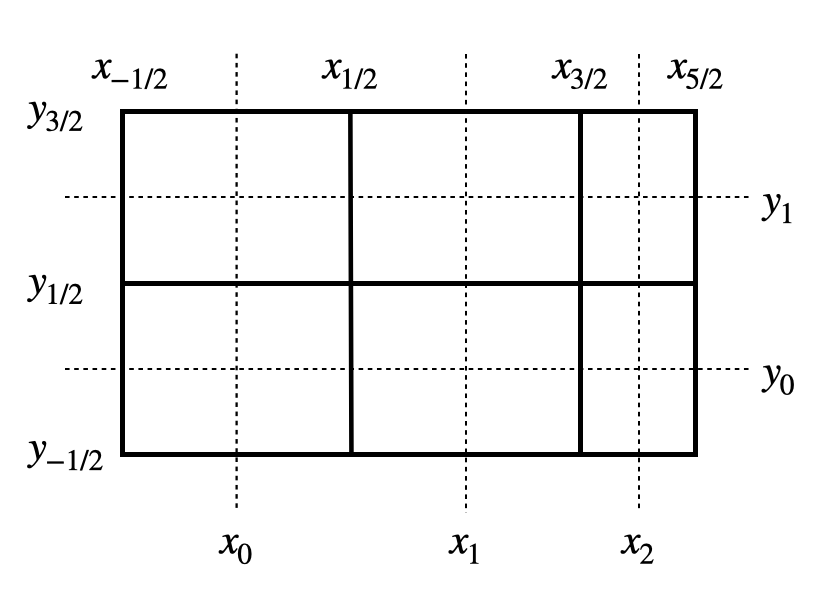
\includegraphics[width=0.5\textwidth]{../../common/figures/porosity_mapper.png}
    \caption{Cartesian grid for the definition of the \texttt{buildings.txt} file. In this case, the file should have 7 lines: header and 6 lines corresponding to each position ($x_i$, $y_j$). The $h$-value for each of theses positions corresponds to the building average height on the rectangle ($x_{i-1/2}$, $x_{i+1/2}$)$\times$($y_{i-1/2}$,$y_{i+1/2}$).}
    \label{fig:porosity_mapping}
\end{figure}

\subsection{Format description: footprint}
This format consists in a list of polygon coordinates corresponding to the building spatial footprints.

The first line is the header containing "x1 y1 … xn yn".
Then, each line describes one building has the following format:
\begin{lstlisting}
<x_1> <y_1> ... <x_i> <y_i> ... <-h> \end{lstlisting}
where $x_i$, $y_i$ are the coordinates of the $i^{th}$ vertice of the building footprint, and -h is optional and is the heigh of the building preceded by a minus sign (used for DDP).
